\section{Model Establishment and Solution}

\subsection{Question 1: Observable Region and Optimal Station}\label{sec:q1}

\subsubsection{Model}

Let $p=(x,y)$ be a candidate station (the vehicle-disc center) and $T$ an alert with
ground projection $T_p$ and height $H$. The observable region
$\mathcal{F}_T=\mathcal{C}_{\mathrm{clr}}\cap\mathcal{C}_{\mathrm{los}}\cap\mathcal{C}_{\mathrm{elev}}$
is the intersection of three constraint sets.

\textbf{(i) Clearance.} The disc of radius $1.5$ m must not penetrate the field boundary
or any building footprint $B_j=[x_{j0},x_{j1}]\times[y_{j0},y_{j1}]$:
\begin{equation}\label{eq:clr}
1.5\le x,y\le98.5,\qquad
\operatorname{dist}\bigl(p,B_j\bigr)=\Bigl\|\bigl(|p-c_j|-s_j\bigr)^{+}\Bigr\|\ge1.5,
\end{equation}
where $c_j$ and $s_j=(s_{jx},s_{jy})$ are the center and half-sizes of $B_j$; equivalently
$p$ must lie outside the Minkowski inflation of every footprint by $1.5$ m
(Fig.~\ref{fig:schematic}b, orange).

\textbf{(ii) Line of sight.} The sightline from $(p,2)$ to $(T_p,H)$ is blocked by
building $B_j$ (height $h_j$) if its horizontal projection meets $B_j$ while its height
there is at most $h_j$; with $\lambda\in[0,1]$ parametrizing the horizontal segment
$p\to T_p$,
\begin{equation}\label{eq:los}
\exists\,\lambda:\; q(\lambda)\in B_j,\;\; z(\lambda)=2+(H-2)\lambda\le h_j ,
\end{equation}
and \emph{tangency counts as blocked} (closed-set test). Because $H>h_j$ for all $j$,
blocking requires $\lambda\le(h_j-2)/(H-2)$: only stations on the far side of a building,
within the ground shadow wedge of the target, lose their sightline.

\textbf{(iii) Elevation.} With $r=\|p-T_p\|$ the horizontal distance and camera height
$2\,\mathrm{m}$, the elevation angle $e=\arctan\bigl((H-2)/r\bigr)$ must lie in
$[-10^\circ,80^\circ]$. Since $H>2$, $e>0$ always, so the binding condition is
\begin{equation}\label{eq:elev}
r\;\ge\;r_{80}\;\triangleq\;\frac{H-2}{\tan 80^\circ}.
\end{equation}

The optimization problem is
\begin{equation}\label{eq:q1opt}
\min_{p\in\mathcal{F}_{T}}\; r(p)=\|p-T_p\| .
\end{equation}
Equation~\eqref{eq:elev} immediately gives the \emph{a priori lower bound} $r\ge r_{80}$;
the optimum attains it iff the circle $\|p-T_p\|=r_{80}$ has a nonempty feasible arc.

\subsubsection{Algorithm}

The region is computed on a $0.1$-m grid over $[1.5,98.5]^2$ (a standard rasterization
approach \cite{deberg2008}): each grid point is tested against
Eq.~\eqref{eq:clr}--\eqref{eq:elev} (LOS uses exact segment--rectangle intersection with
closed endpoints), components are labeled, and the boundary is refined by a $0.02$-m
local search around sign changes. Independently, the \emph{critical circle}
$\|p-T_p\|=r_{80}$ is traced analytically: each station azimuth $\phi$ is tested against
clearance and LOS, yielding the feasible arc(s) with the cause of each endpoint---this
audit certifies whether Eq.~\eqref{eq:q1opt}'s lower bound is attained.

Tie-breaking over the optimal arc is declared as part of the model, in priority order:
\textbf{(1)} a hard clearance margin of $0.10\,\mathrm{m}$ beyond the $1.5$-m vehicle
buffer (boundary robustness); \textbf{(2)} minimize the designated vehicle's
\emph{mission-cycle time} from its standby position---travel $+$ slew $+$ 5-s joint
observation $+$ reset $=$ travel $+2\tau+5\,\mathrm{s}$, since the reset mirrors the
slew---with the nearest standby vehicle designated as the observer for each target
(V4 for T1, V3 for T2, V2 for T3); \textbf{(3)} ties: larger clearance margin, then
distance to the dispatch center $O$, then azimuth. On the $r_{80}$-arc every station
has $\mathrm{tilt}=80^\circ$, so $\tau=2.667\,\mathrm{s}$ whenever
$|\mathrm{wrap}(\mathrm{pan})|\le80^\circ$ and the cycle reduces to
$\mathrm{travel}+10.33\,\mathrm{s}$---the rule selects the arc point closest to the
designated vehicle.

\subsubsection{Results}

\begin{table}[!htb]\centering\footnotesize\setlength{\tabcolsep}{4pt}
\caption{Observable regions and min-$r$ optimal stations (grid $0.1$ m; angles on the
$r_{80}$-circle measured from the target projection, CCW from east). Stations are
reported to six decimals---see the printed-precision note below.}
\label{tab:q1opt}
\begin{tabular}{lccc}
\toprule
 & T1 & T2 & T3 \\
\midrule
$r_{80}$ (m) & 7.5821 & 5.8188 & 9.3453 \\
feasible arc on $r_{80}$-circle & $[236.90^\circ,160.74^\circ]$ & $[59.66^\circ,244.24^\circ]$ & full circle \\
arc span / endpoint cause & $283.84^\circ$ / clearance & $184.58^\circ$ / LOS, clearance & $360^\circ$ / -- \\
area of $\mathcal{F}_T$ (m$^2$) & 5628.7 & 6432.5 & 5484.8 \\
connected components & 1 & 1 & 1 \\
designated vehicle & V4 & V3 & V2 \\
optimal station $(x,y)$ & $(83.324405,\,62.533128)$ & $(10.018434,\,78.230390)$ & $(58.212324,\,4.091465)$ \\
pan / tilt ($^\circ$) & $80.0\,/\,80.0$ & $280.0\,/\,80.0$ & $80.0\,/\,80.0$ \\
slew $=$ reset (s) & 2.667 & 2.667 & 2.667 \\
mission cycle (s) & 12.731 & 13.243 & 20.456 \\
clearance beyond buffer (m) & 2.824 & 0.730 & 2.591 \\
\bottomrule
\end{tabular}
\end{table}

The minimum $r^{*}=r_{80}$ is attained for all three targets: T1's critical circle
survives over a $283.84^\circ$ arc, T2's over $184.58^\circ$ (one end LOS-limited, the
other clearance-limited), and T3's entire circle is feasible ($H=55$ clears every
building). Rule (2) selects, on each arc, the point closest to the designated
vehicle's standby position: V4 for T1 (azimuth $260.0^\circ$), V3 for T2
($100.0^\circ$---the edge of the constant-slew sector, where travel toward V3 is
shortest), and V2 for T3 ($260.0^\circ$). Table~\ref{tab:q1opt} lists the stations;
all three sit \emph{exactly} on the $80^\circ$ elevation boundary---inherent to the
objective, since $Q=1/r$ is maximal only on the $r_{80}$-circle---feasible on the
closed set, with robustness examined in Section~\ref{sec:sens}.

\emph{Printed precision.} The table reports six decimals deliberately: all three
stations sit at exactly $80.000000^\circ$ elevation (T2 additionally at the edge of
the constant-slew sector), so a four-decimal rounding can push the printed point
$10^{-5}\,\mathrm{m}$ inside the elevation boundary and a strict re-check would---wrongly---reject
it. Deployments should use the six-decimal values (or the exact construction
$p^{*}=T_p+r_{80}(\cos\varphi^{*},\sin\varphi^{*})$); every reported station carries
the $0.10$-m clearance margin of rule (1), and a $0.5^\circ$ step along the arc into
the interior is strictly feasible in both of our implementations with \emph{identical}
$Q$, since every arc point has $r=r_{80}$.

\emph{Alternative tie-break (nearest to $O$).} An earlier draft declared a different
rule---minimize the distance to the dispatch center over the arc---which selects
$(80.500050,\,63.648619)$ for T1 at the clearance-tangent arc endpoint (mission cycle
$13.22\,\mathrm{s}$, clearance margin $0.0004\,\mathrm{m}$). Both rules are reasonable
under the problem statement; the mission-cycle rule is adopted because the problem's
objective is \emph{rapid} deployment and it matches the convention used in Q2(1), and
the coexistence of the two outcomes on the same arc---identical $Q$, cycle differing
by $0.49\,\mathrm{s}$---confirms the flat-optimum structure.

\begin{figure}[!htb]\centering
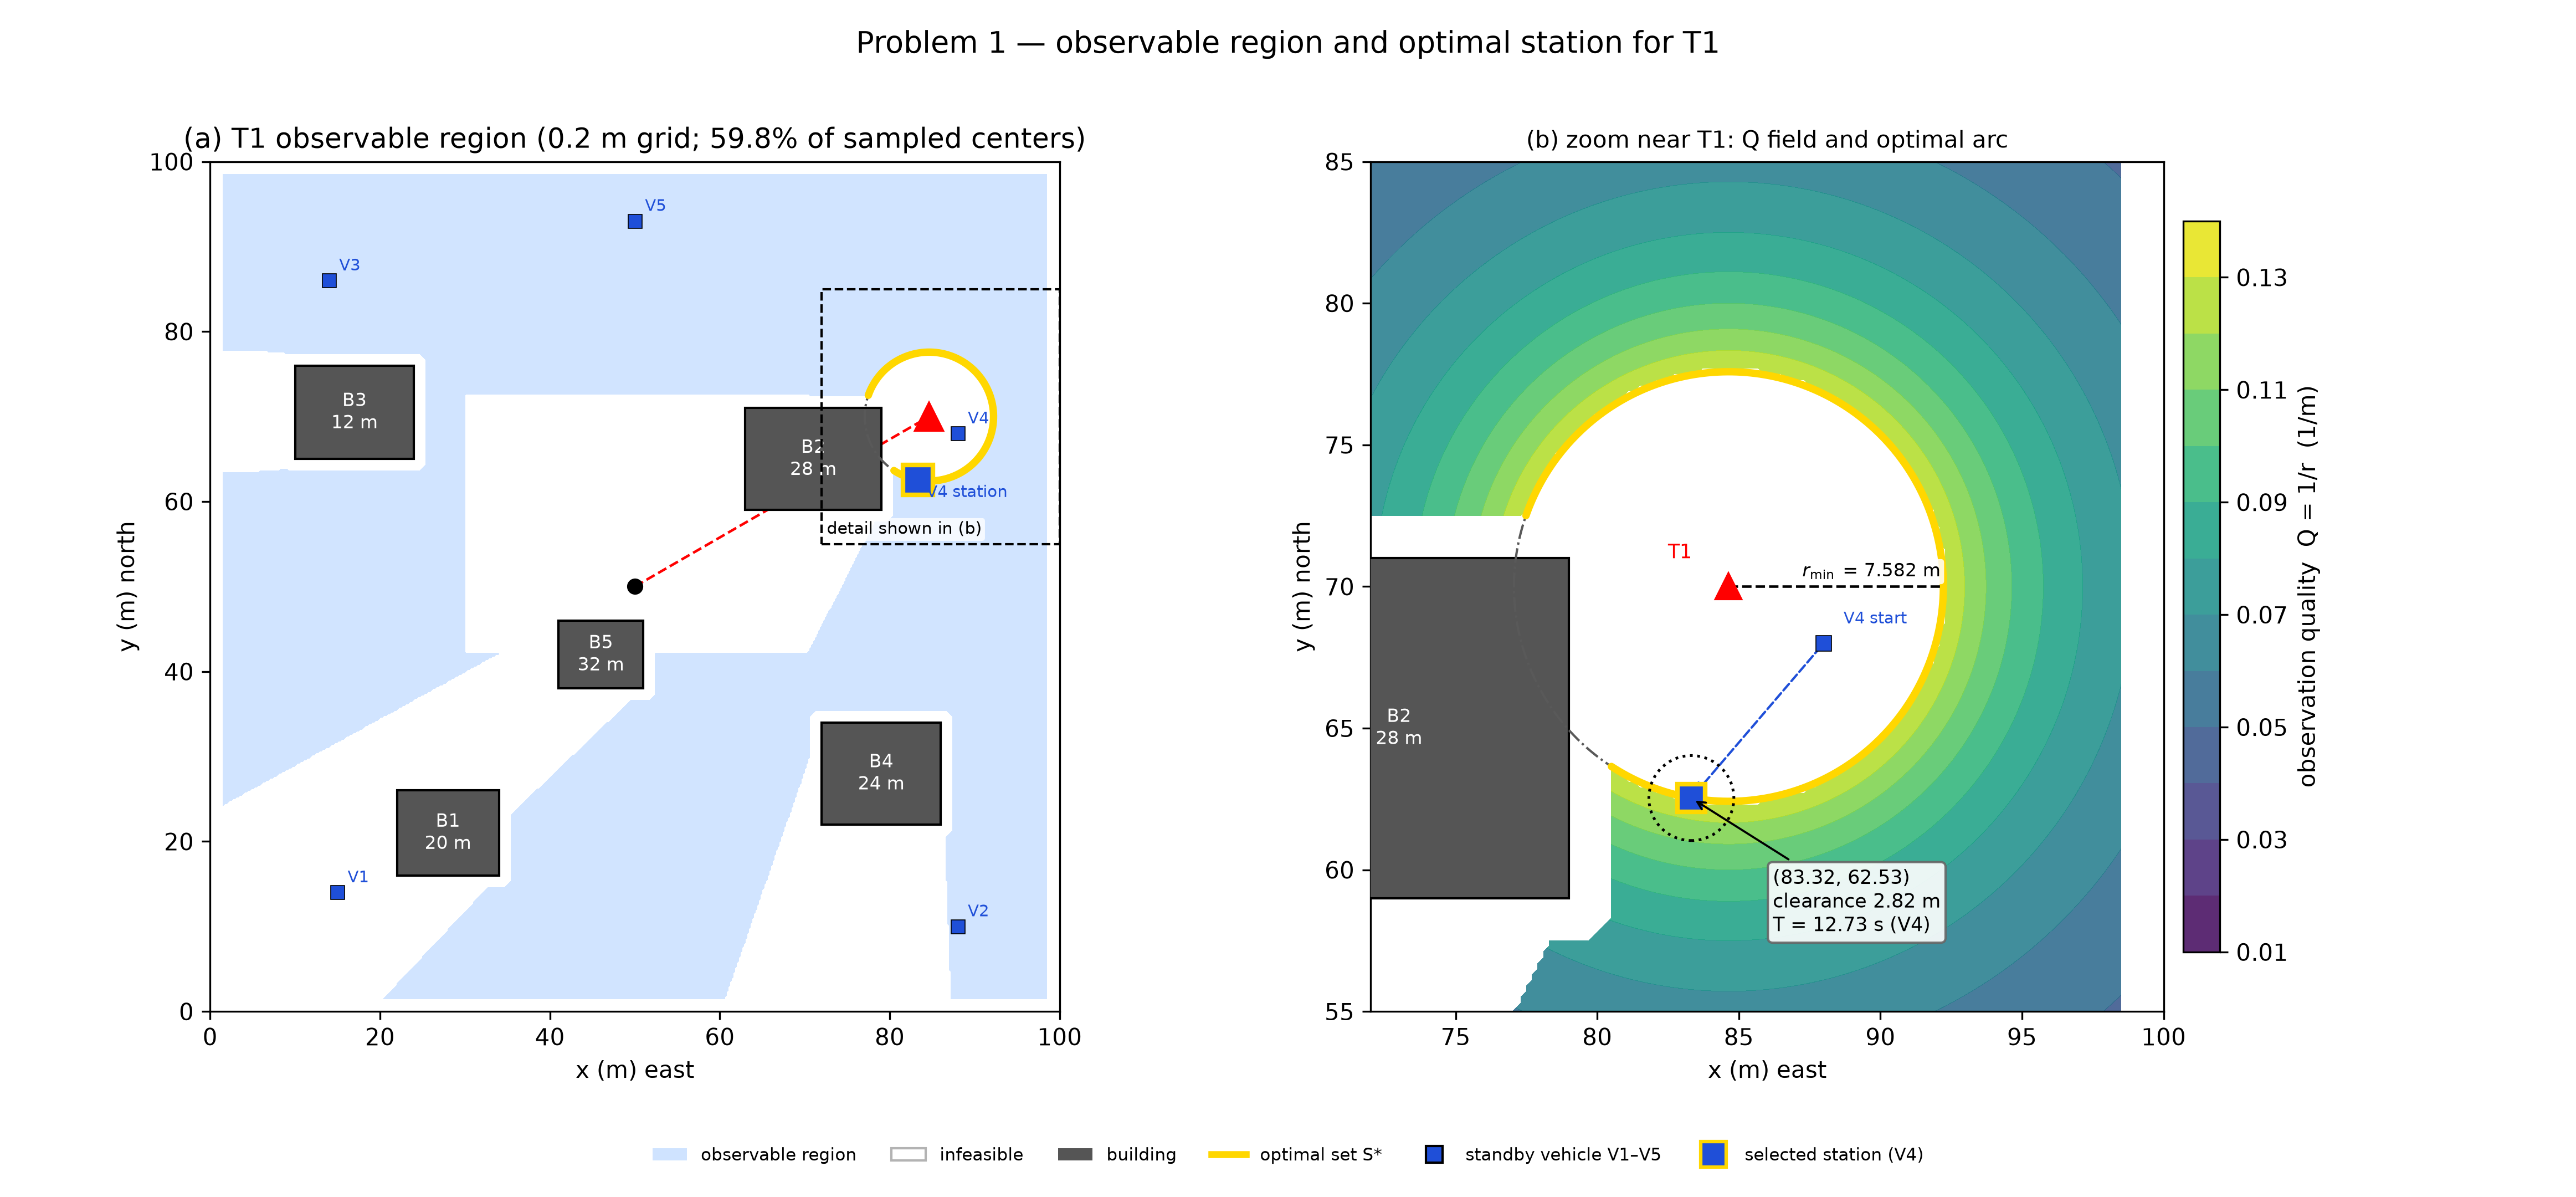
\includegraphics[width=\textwidth]{fig_q1_T1_region.png}
\caption{T1 observable region (left: $0.2$-m raster, $59.8\%$ of sampled centers;
right: zoom on the quality field $Q=1/r$). The gold arc is the optimal set
$S^{*}$---every point of it attains $r^{*}=7.5821$ m ($Q^{*}=0.1319$ m$^{-1}$); the
blocked sector ($160.74^\circ$--$236.90^\circ$) is the $B_2$ shadow. The selected
station for the designated vehicle V4 (square, with its $1.5$-m disk) carries a
$2.82$-m clearance margin, and the annotation reports V4's full mission cycle.}
\label{fig:q1t1}
\end{figure}
\begin{figure}[!htb]\centering
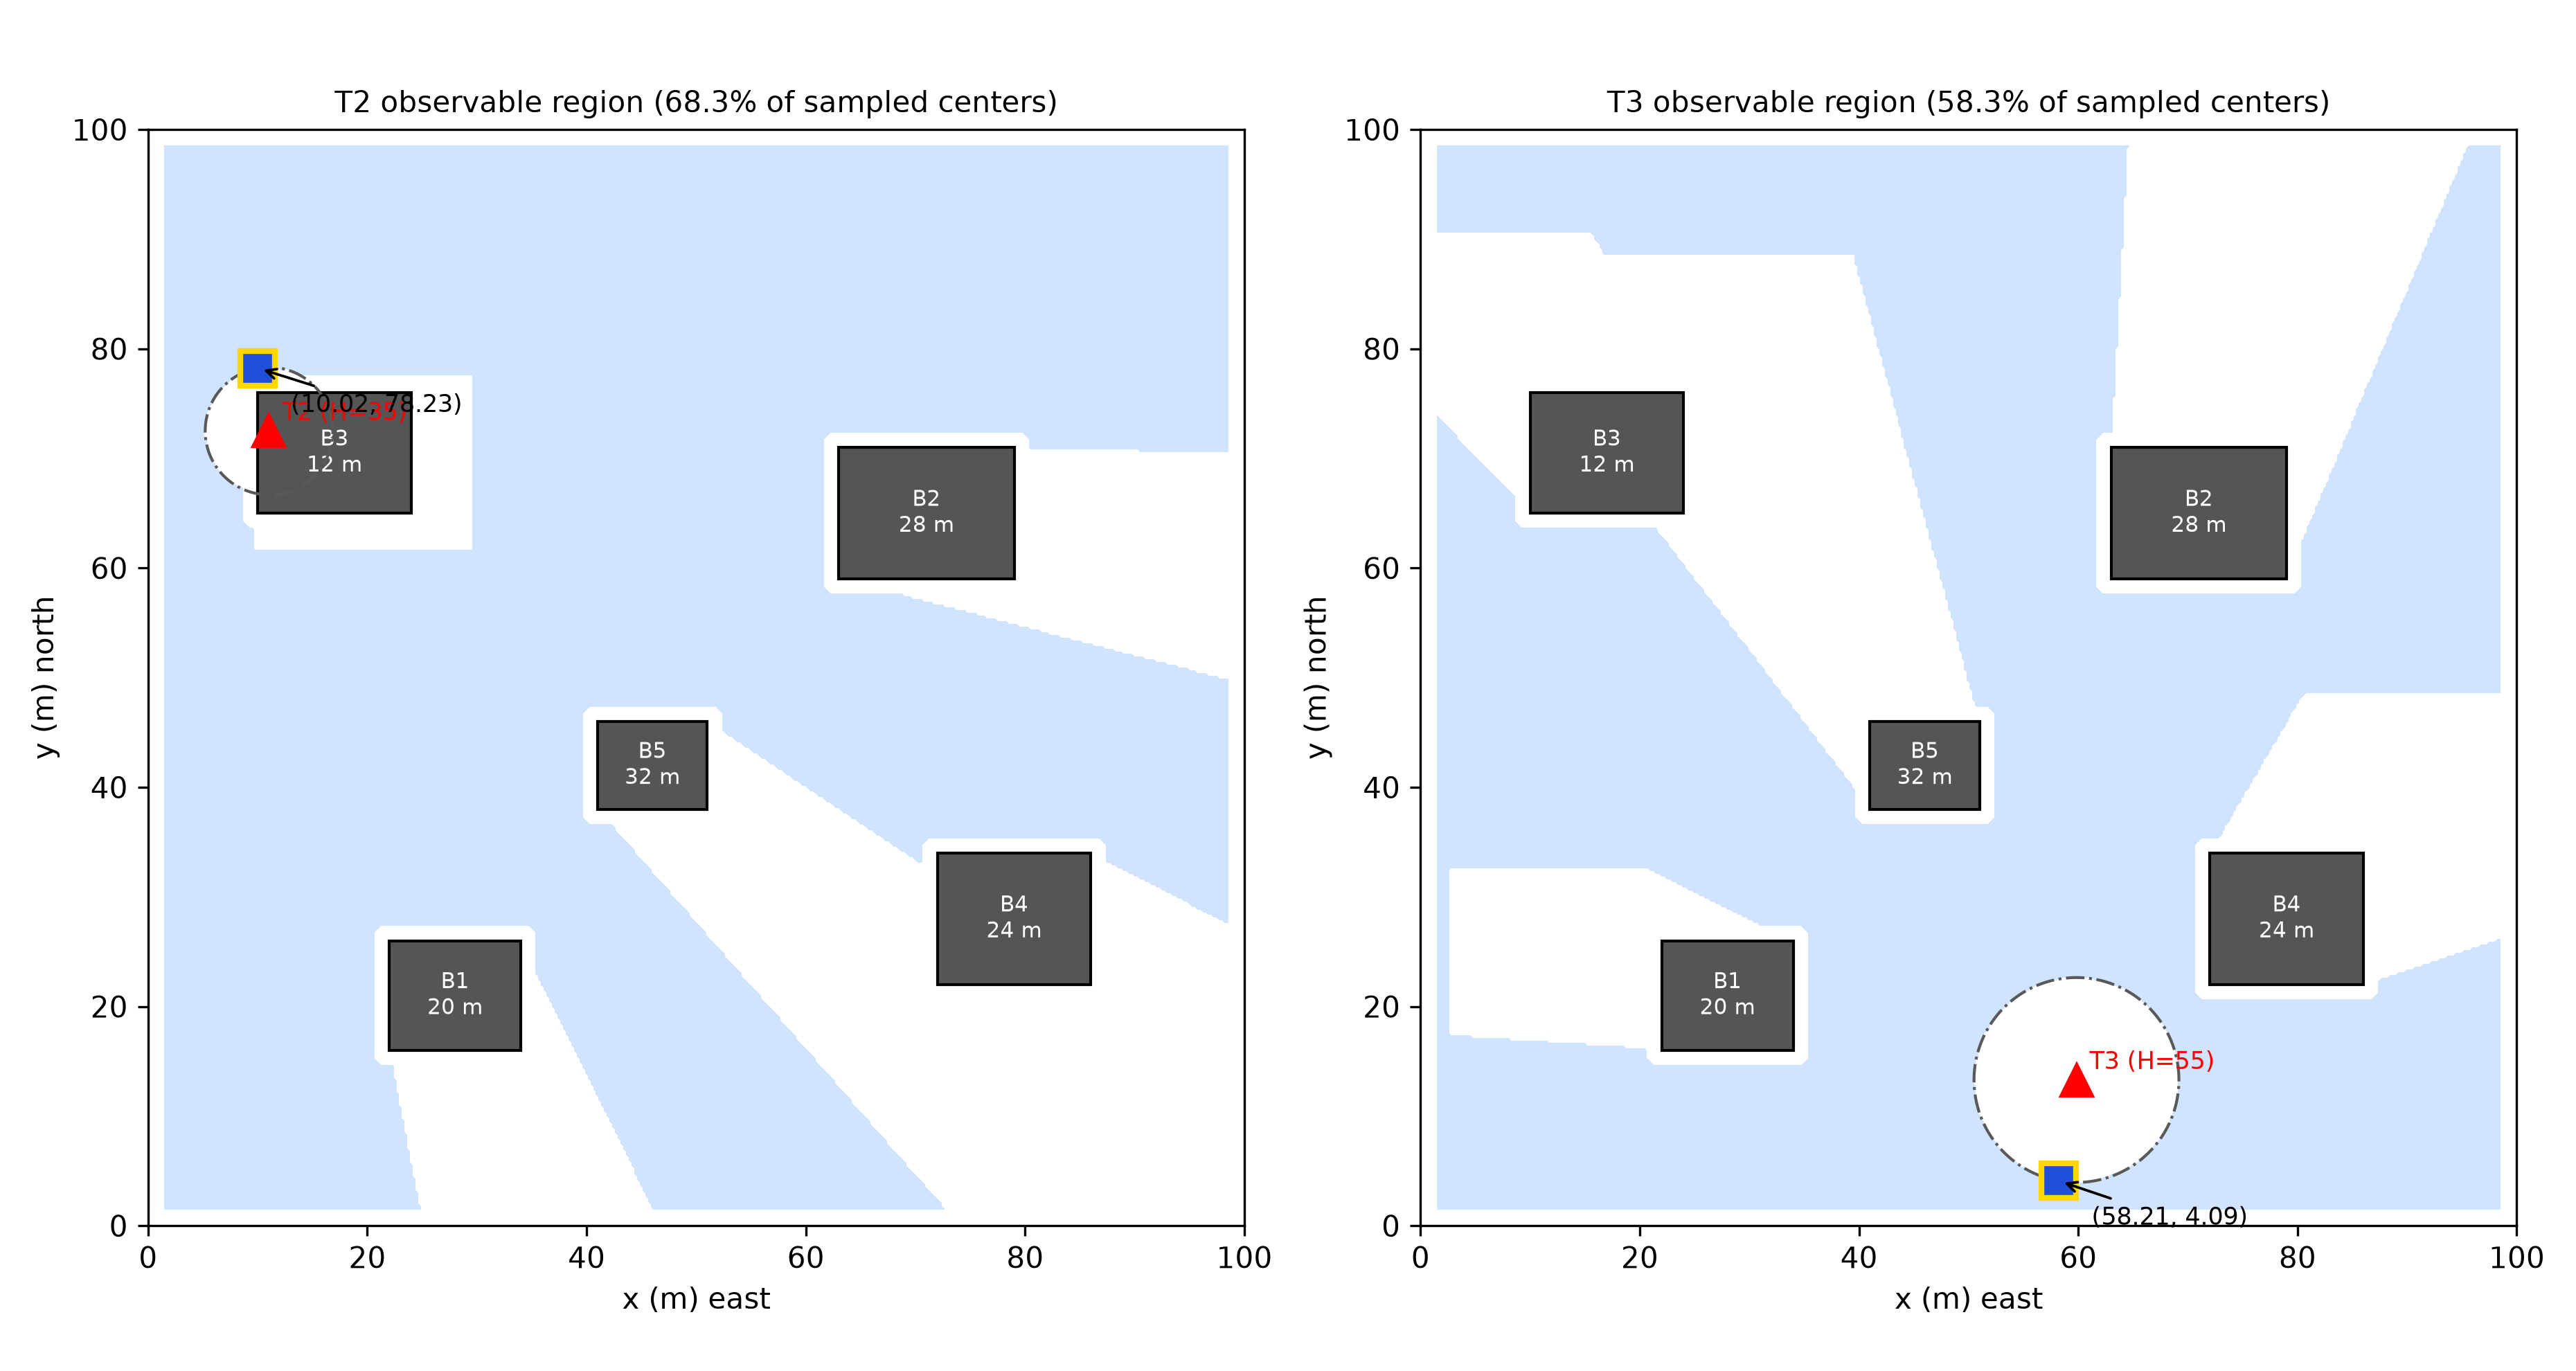
\includegraphics[width=0.78\textwidth]{fig_q1_T2_T3_regions.png}
\caption{Observable regions of T2 (left) and T3 (right) at $0.25$-m resolution with
the selected stations. T2 is pinched by $B_3$'s shadow and clearance, while T3 (the
tallest target) keeps its full elevation circle; all three selected stations
lie on the elevation circle closest to their designated vehicle.}
\label{fig:q1t23}
\end{figure}

Figures~\ref{fig:q1t1} and~\ref{fig:q1t23} confirm the mechanism predicted in Section~2.2: elevation removes
a disc around each target, clearance removes collars around buildings and the boundary,
and LOS removes wedges only on the far side of buildings relative to the (high)
target---for T2 the wedge is large because the target hovers low ($35$ m) above $B_3$,
while T3 loses nothing to LOS. The regions are all single components of areas
$5.5$--$6.4\times10^3\,\mathrm{m}^2$ ($55$--$64\%$ of the field), so station placement
has ample freedom for the later questions.

\subsubsection{Validation}

Four checks close Q1. First, at each chosen station all three constraints were
re-evaluated pointwise: elevations equal exactly $80.000000^\circ$ (the objective
boundary, inherent to $Q=1/r$), and the clearance margins of rule (1) are
$2.82/0.73/2.59\,\mathrm{m}$ beyond the buffer for T1/T2/T3, as designed. Second,
halving and doubling the grid resolution changes the region areas by at most $0.23\%$
(T1: $5628.7\,\mathrm{m}^2$ at $0.1$ m, $5619.6$ at $0.05$ m, $5607.8$ at $0.2$ m), so
the reported areas are resolution-stable. Third, the analytic critical-circle trace
reproduces the grid's inner (elevation) boundary and its feasible arcs exactly,
certifying that Eq.~\eqref{eq:q1opt}'s lower bound is genuinely attained rather than
grid-limited. \emph{Conclusion: the region computation and the optimum are mutually
consistent, and the optimum is exact on the continuous feasible set.}
